% Autor: Francisco Javier Barranco Tena
% Validación de los modelos
% Alt + z o Option + z para activar el word wrap en Visual Studio Code

La validación es una parte fundamental en el desarrollo de modelos de aprendizaje automático, ya que nos permite comprobar si nuestro modelo es capaz de generalizar bien a datos que no ha visto antes. En esta sección se va a explicar cómo se ha llevado a cabo la validación de los modelos de detección de estado del pavimento desarrollados en este TFG. Comenzaremos explicando que es la validación cruzada y por qué es importante. Después, se explicará cómo se ha llevado a cabo la validación cruzada en este TFG y se mostrarán los resultados obtenidos.

\subsection{Validación cruzada (Cross-validation)}
La validación cruzada es una técnica que se utiliza para evaluar la capacidad de generalización de un modelo de aprendizaje automático. Consiste en dividir el conjunto de datos en $k$ subconjuntos, llamados \textit{folds}, y entrenar el modelo $k$ veces, cada vez utilizando un subconjunto distinto como conjunto de validación y el resto de subconjuntos como conjunto de entrenamiento. De esta forma, se obtienen $k$ métricas de evaluación distintas, una por cada iteración, y se pueden calcular métricas de evaluación globales como la media y la desviación estándar de las métricas de evaluación de cada iteración. En la figura \ref{fig:cross_validation} se puede ver un esquema de cómo se lleva a cabo la validación cruzada.

% Añadir la imagen K-fold_cross_validation.jpg de la carpeta img
\begin{figure}[H]
    \centering
    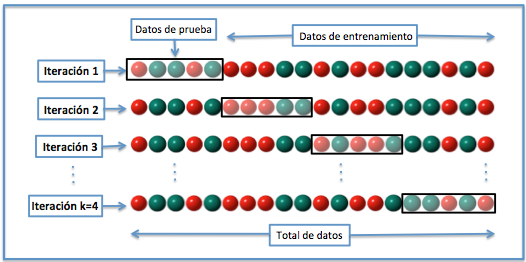
\includegraphics[width=0.8\textwidth]{img/K-fold_cross_validation.jpg}
    \caption{Esquema de cómo se lleva a cabo la validación cruzada. \cite{KFoldCV_image}}
    \label{fig:cross_validation}
\end{figure}

\subsection{Validación cruzada propuesta}
En este TFG se ha llevado a cabo una validación cruzada de 4 \textit{folds} para evaluar los modelos. Es decir, cada iteración se ha entrenado con un 75\% de los datos anotados y se ha validado con el 25\% restante. Para dividir los datos hemos separado las carpetas de train de cada región en 4 subcarpetas fold\_0, fold\_1, fold\_2 y fold\_3. Cada una de estas subcarpetas contiene un 25\% de las imágenes y anotaciones de la carpeta de train correspondiente. De esta forma, cuando vamos a crear el fichero \textit{.yaml} que contiene la información de los datos de entrenamiento y validación, simplemente concatenamos las rutas de las subcarpetas fold\_0, fold\_1, fold\_2 y fold\_3 para obtener los datos de entrenamiento y validación de cada iteración. Además de esta forma nos aseguramos que al entrenar con los datos de varias regiones, el modelo entrena con datos de todas las regiones de forma proporcional al número de imágenes de cada región. Esto es importante para que el modelo no se sobre ajuste a una región en concreto y sea capaz de generalizar bien a datos de todas las regiones. Véase como ejemplo de un fichero \textit{.yaml} en la figura \ref{fig:yaml_example}.

% Añadir el código de un .yaml como ejemplo
\begin{figure}[H]
    \centering
    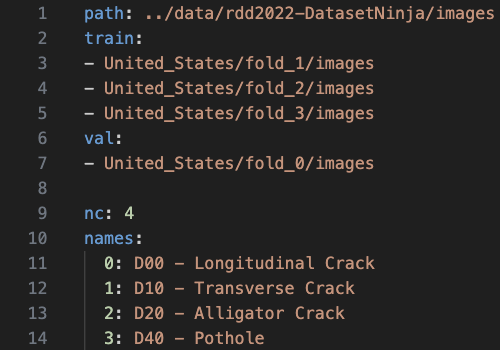
\includegraphics[width=0.8\textwidth]{img/yaml_example.png}
    \caption{Ejemplo de un fichero \textit{.yaml} que contiene la información de los datos de entrenamiento y validación para entrenar un modelo YOLO con las imágenes y anotaciones de EEUU de la CRDDC2022.}
    \label{fig:yaml_example}
\end{figure}

Otra consideración importante cuando creamos los \textit{folds} es que las imágenes de una misma secuencia de imagenes, por ejemplo las imágenes de una misma calle, contienen información muy similar. Por lo tanto, podemos barajar (shuffle) las imágenes antes de separar en folds para maximizar la información que hay en cada fold y de esta forma aumentar la capacidad de generalización de nuestro modelo. La desventaja de esta técnica es que dos imágenes pertenecientes a una misma secuencia de imágenes pueden acabar una en el conjunto de entrenamiento y otra en el conjunto de validación, lo que puede hacer que el modelo se sobre ajuste a esta secuencia de imágenes, ya que la puntuación de precisión y recall será muy alta al ser las imágenes muy parecidas. No obstante, en este TFG se ha decidido barajar las imágenes antes de separar en folds, ya que se considera que la ventaja de maximizar la información en cada fold es más importante que la desventaja de que el modelo se sobre ajuste a una secuencia de imágenes.